\documentclass{standalone}

\usepackage[T1]{fontenc}
\usepackage[utf8]{inputenc}
\usepackage{eulervm}
\usepackage{amsmath}
\usepackage{bm}
\usepackage{tikz}
\usepackage{environ}

\usetikzlibrary{fit}
\usetikzlibrary{patterns}
\usetikzlibrary{arrows}

\usepackage{color}

\definecolor{Comment}{RGB}{97,161,176}

\definecolor{btfGreen}{RGB}{51,160,44}
\definecolor{btfRed}{RGB}{190,60,90}

\definecolor{bleuUni}{RGB}{0, 157, 224}
\definecolor{marronUni}{RGB}{68, 58, 49}
\definecolor{grayMarronUni}{RGB}{60, 60, 60}
\definecolor{grayBleuUni}{RGB}{118, 118, 118}

\definecolor{bluecite}{HTML}{009DE0}

\definecolor{Paired-2}{RGB}{166,206,227}
\definecolor{Paired-1}{RGB}{31,120,180}
\definecolor{Paired-4}{RGB}{178,223,138}
\definecolor{Paired-3}{RGB}{51,160,44}
\definecolor{Paired-6}{RGB}{251,154,153}
\definecolor{Paired-5}{RGB}{227,26,28}
\definecolor{Paired-8}{RGB}{253,191,111}
\definecolor{Paired-7}{RGB}{255,127,0}
\definecolor{Paired-10}{RGB}{202,178,214}
\definecolor{Paired-9}{RGB}{106,61,154}
\definecolor{Paired-12}{RGB}{255,255,153}
\definecolor{Paired-11}{RGB}{177,89,40}
\definecolor{Accent-1}{RGB}{127,201,127}
\definecolor{Accent-2}{RGB}{190,174,212}
\definecolor{Accent-3}{RGB}{253,192,134}
\definecolor{Accent-4}{RGB}{255,255,153}
\definecolor{Accent-5}{RGB}{56,108,176}
\definecolor{Accent-6}{RGB}{240,2,127}
\definecolor{Accent-7}{RGB}{191,91,23}
\definecolor{Accent-8}{RGB}{102,102,102}
\definecolor{Spectral-1}{RGB}{158,1,66}
\definecolor{Spectral-2}{RGB}{213,62,79}
\definecolor{Spectral-3}{RGB}{244,109,67}
\definecolor{Spectral-4}{RGB}{253,174,97}
\definecolor{Spectral-5}{RGB}{254,224,139}
\definecolor{Spectral-6}{RGB}{255,255,191}
\definecolor{Spectral-7}{RGB}{230,245,152}
\definecolor{Spectral-8}{RGB}{171,221,164}
\definecolor{Spectral-9}{RGB}{102,194,165}
\definecolor{Spectral-10}{RGB}{50,136,189}
\definecolor{Spectral-11}{RGB}{94,79,162}
\definecolor{Set1-1}{RGB}{228,26,28}
\definecolor{Set1-2}{RGB}{55,126,184}
\definecolor{Set1-3}{RGB}{77,175,74}
\definecolor{Set1-4}{RGB}{152,78,163}
\definecolor{Set1-5}{RGB}{255,127,0}
\definecolor{Set1-6}{RGB}{255,255,51}
\definecolor{Set1-7}{RGB}{166,86,40}
\definecolor{Set1-8}{RGB}{247,129,191}
\definecolor{Set1-9}{RGB}{153,153,153}
\definecolor{Set2-1}{RGB}{102,194,165}
\definecolor{Set2-2}{RGB}{252,141,98}
\definecolor{Set2-3}{RGB}{141,160,203}
\definecolor{Set2-4}{RGB}{231,138,195}
\definecolor{Set2-5}{RGB}{166,216,84}
\definecolor{Set2-6}{RGB}{255,217,47}
\definecolor{Set2-7}{RGB}{229,196,148}
\definecolor{Set2-8}{RGB}{179,179,179}
\definecolor{Dark2-1}{RGB}{27,158,119}
\definecolor{Dark2-2}{RGB}{217,95,2}
\definecolor{Dark2-3}{RGB}{117,112,179}
\definecolor{Dark2-4}{RGB}{231,41,138}
\definecolor{Dark2-5}{RGB}{102,166,30}
\definecolor{Dark2-6}{RGB}{230,171,2}
\definecolor{Dark2-7}{RGB}{166,118,29}
\definecolor{Dark2-8}{RGB}{102,102,102}
\definecolor{Reds-1}{RGB}{255,245,240}
\definecolor{Reds-2}{RGB}{254,224,210}
\definecolor{Reds-3}{RGB}{252,187,161}
\definecolor{Reds-4}{RGB}{252,146,114}
\definecolor{Reds-5}{RGB}{251,106,74}
\definecolor{Reds-6}{RGB}{239,59,44}
\definecolor{Reds-7}{RGB}{203,24,29}
\definecolor{Reds-8}{RGB}{165,15,21}
\definecolor{Reds-9}{RGB}{103,0,13}
\definecolor{Greens-1}{RGB}{247,252,245}
\definecolor{Greens-2}{RGB}{229,245,224}
\definecolor{Greens-3}{RGB}{199,233,192}
\definecolor{Greens-4}{RGB}{161,217,155}
\definecolor{Greens-5}{RGB}{116,196,118}
\definecolor{Greens-6}{RGB}{65,171,93}
\definecolor{Greens-7}{RGB}{35,139,69}
\definecolor{Greens-8}{RGB}{0,109,44}
\definecolor{Greens-9}{RGB}{0,68,27}
\definecolor{Blues-1}{RGB}{247,251,255}
\definecolor{Blues-2}{RGB}{222,235,247}
\definecolor{Blues-3}{RGB}{198,219,239}
\definecolor{Blues-4}{RGB}{158,202,225}
\definecolor{Blues-5}{RGB}{107,174,214}
\definecolor{Blues-6}{RGB}{66,146,198}
\definecolor{Blues-7}{RGB}{33,113,181}
\definecolor{Blues-8}{RGB}{8,81,156}
\definecolor{Blues-9}{RGB}{8,48,107}


\begin{document}
  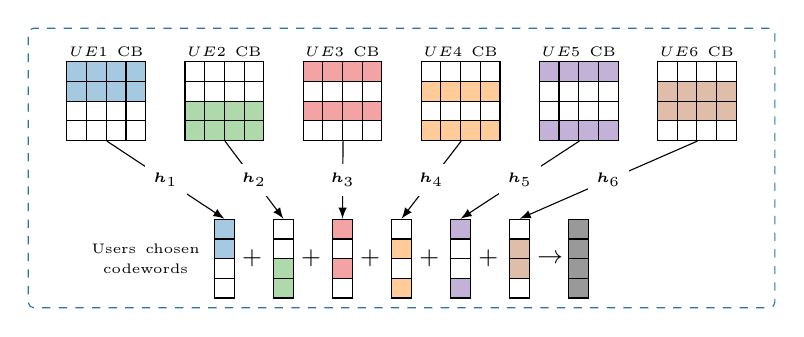
\begin{tikzpicture}[baseline]
    \tikzset{ cbemp/.style={draw=black, minimum width=0.25cm, minimum height=0.25cm, text=black, fill=white       } }
    \tikzset{ cbue1/.style={draw=black, minimum width=0.25cm, minimum height=0.25cm, text=black, fill=Paired-1!40 } }
    \tikzset{ cbue2/.style={draw=black, minimum width=0.25cm, minimum height=0.25cm, text=black, fill=Paired-3!40 } }
    \tikzset{ cbue3/.style={draw=black, minimum width=0.25cm, minimum height=0.25cm, text=black, fill=Paired-5!40 } }
    \tikzset{ cbue4/.style={draw=black, minimum width=0.25cm, minimum height=0.25cm, text=black, fill=Paired-7!40 } }
    \tikzset{ cbue5/.style={draw=black, minimum width=0.25cm, minimum height=0.25cm, text=black, fill=Paired-9!40 } }
    \tikzset{ cbue6/.style={draw=black, minimum width=0.25cm, minimum height=0.25cm, text=black, fill=Paired-11!40} }
    \tikzset{ cbadd/.style={draw=black, minimum width=0.25cm, minimum height=0.25cm, text=black, fill=black!40    } }

    \newcommand\yshft{2.00}

    \node[cbemp] (ue1_cb_0_0) at (0.00+0.00, \yshft+0.00) {};
    \node[cbemp] (ue1_cb_1_0) at (0.00+0.25, \yshft+0.00) {};
    \node[cbemp] (ue1_cb_2_0) at (0.00+0.50, \yshft+0.00) {};
    \node[cbemp] (ue1_cb_3_0) at (0.00+0.75, \yshft+0.00) {};
    \node[cbemp] (ue1_cb_0_1) at (0.00+0.00, \yshft+0.25) {};
    \node[cbemp] (ue1_cb_1_1) at (0.00+0.25, \yshft+0.25) {};
    \node[cbemp] (ue1_cb_2_1) at (0.00+0.50, \yshft+0.25) {};
    \node[cbemp] (ue1_cb_3_1) at (0.00+0.75, \yshft+0.25) {};
    \node[cbue1] (ue1_cb_0_2) at (0.00+0.00, \yshft+0.50) {};
    \node[cbue1] (ue1_cb_1_2) at (0.00+0.25, \yshft+0.50) {};
    \node[cbue1] (ue1_cb_2_2) at (0.00+0.50, \yshft+0.50) {};
    \node[cbue1] (ue1_cb_3_2) at (0.00+0.75, \yshft+0.50) {};
    \node[cbue1] (ue1_cb_0_3) at (0.00+0.00, \yshft+0.75) {};
    \node[cbue1] (ue1_cb_1_3) at (0.00+0.25, \yshft+0.75) {};
    \node[cbue1] (ue1_cb_2_3) at (0.00+0.50, \yshft+0.75) {};
    \node[cbue1] (ue1_cb_3_3) at (0.00+0.75, \yshft+0.75) {};

    \node[cbue2] (ue2_cb_0_0) at (1.50+0.00, \yshft+0.00) {};
    \node[cbue2] (ue2_cb_1_0) at (1.50+0.25, \yshft+0.00) {};
    \node[cbue2] (ue2_cb_2_0) at (1.50+0.50, \yshft+0.00) {};
    \node[cbue2] (ue2_cb_3_0) at (1.50+0.75, \yshft+0.00) {};
    \node[cbue2] (ue2_cb_0_1) at (1.50+0.00, \yshft+0.25) {};
    \node[cbue2] (ue2_cb_1_1) at (1.50+0.25, \yshft+0.25) {};
    \node[cbue2] (ue2_cb_2_1) at (1.50+0.50, \yshft+0.25) {};
    \node[cbue2] (ue2_cb_3_1) at (1.50+0.75, \yshft+0.25) {};
    \node[cbemp] (ue2_cb_0_2) at (1.50+0.00, \yshft+0.50) {};
    \node[cbemp] (ue2_cb_1_2) at (1.50+0.25, \yshft+0.50) {};
    \node[cbemp] (ue2_cb_2_2) at (1.50+0.50, \yshft+0.50) {};
    \node[cbemp] (ue2_cb_3_2) at (1.50+0.75, \yshft+0.50) {};
    \node[cbemp] (ue2_cb_0_3) at (1.50+0.00, \yshft+0.75) {};
    \node[cbemp] (ue2_cb_1_3) at (1.50+0.25, \yshft+0.75) {};
    \node[cbemp] (ue2_cb_2_3) at (1.50+0.50, \yshft+0.75) {};
    \node[cbemp] (ue2_cb_3_3) at (1.50+0.75, \yshft+0.75) {};

    \node[cbemp] (ue3_cb_0_0) at (3.00+0.00, \yshft+0.00) {};
    \node[cbemp] (ue3_cb_1_0) at (3.00+0.25, \yshft+0.00) {};
    \node[cbemp] (ue3_cb_2_0) at (3.00+0.50, \yshft+0.00) {};
    \node[cbemp] (ue3_cb_3_0) at (3.00+0.75, \yshft+0.00) {};
    \node[cbue3] (ue3_cb_0_1) at (3.00+0.00, \yshft+0.25) {};
    \node[cbue3] (ue3_cb_1_1) at (3.00+0.25, \yshft+0.25) {};
    \node[cbue3] (ue3_cb_2_1) at (3.00+0.50, \yshft+0.25) {};
    \node[cbue3] (ue3_cb_3_1) at (3.00+0.75, \yshft+0.25) {};
    \node[cbemp] (ue3_cb_0_2) at (3.00+0.00, \yshft+0.50) {};
    \node[cbemp] (ue3_cb_1_2) at (3.00+0.25, \yshft+0.50) {};
    \node[cbemp] (ue3_cb_2_2) at (3.00+0.50, \yshft+0.50) {};
    \node[cbemp] (ue3_cb_3_2) at (3.00+0.75, \yshft+0.50) {};
    \node[cbue3] (ue3_cb_0_3) at (3.00+0.00, \yshft+0.75) {};
    \node[cbue3] (ue3_cb_1_3) at (3.00+0.25, \yshft+0.75) {};
    \node[cbue3] (ue3_cb_2_3) at (3.00+0.50, \yshft+0.75) {};
    \node[cbue3] (ue3_cb_3_3) at (3.00+0.75, \yshft+0.75) {};

    \node[cbue4] (ue4_cb_0_0) at (4.50+0.00, \yshft+0.00) {};
    \node[cbue4] (ue4_cb_1_0) at (4.50+0.25, \yshft+0.00) {};
    \node[cbue4] (ue4_cb_2_0) at (4.50+0.50, \yshft+0.00) {};
    \node[cbue4] (ue4_cb_3_0) at (4.50+0.75, \yshft+0.00) {};
    \node[cbemp] (ue4_cb_0_1) at (4.50+0.00, \yshft+0.25) {};
    \node[cbemp] (ue4_cb_1_1) at (4.50+0.25, \yshft+0.25) {};
    \node[cbemp] (ue4_cb_2_1) at (4.50+0.50, \yshft+0.25) {};
    \node[cbemp] (ue4_cb_3_1) at (4.50+0.75, \yshft+0.25) {};
    \node[cbue4] (ue4_cb_0_2) at (4.50+0.00, \yshft+0.50) {};
    \node[cbue4] (ue4_cb_1_2) at (4.50+0.25, \yshft+0.50) {};
    \node[cbue4] (ue4_cb_2_2) at (4.50+0.50, \yshft+0.50) {};
    \node[cbue4] (ue4_cb_3_2) at (4.50+0.75, \yshft+0.50) {};
    \node[cbemp] (ue4_cb_0_3) at (4.50+0.00, \yshft+0.75) {};
    \node[cbemp] (ue4_cb_1_3) at (4.50+0.25, \yshft+0.75) {};
    \node[cbemp] (ue4_cb_2_3) at (4.50+0.50, \yshft+0.75) {};
    \node[cbemp] (ue4_cb_3_3) at (4.50+0.75, \yshft+0.75) {};

    \node[cbue5] (ue5_cb_0_0) at (6.00+0.00, \yshft+0.00) {};
    \node[cbue5] (ue5_cb_1_0) at (6.00+0.25, \yshft+0.00) {};
    \node[cbue5] (ue5_cb_2_0) at (6.00+0.50, \yshft+0.00) {};
    \node[cbue5] (ue5_cb_3_0) at (6.00+0.75, \yshft+0.00) {};
    \node[cbemp] (ue5_cb_0_1) at (6.00+0.00, \yshft+0.25) {};
    \node[cbemp] (ue5_cb_1_1) at (6.00+0.25, \yshft+0.25) {};
    \node[cbemp] (ue5_cb_2_1) at (6.00+0.50, \yshft+0.25) {};
    \node[cbemp] (ue5_cb_3_1) at (6.00+0.75, \yshft+0.25) {};
    \node[cbemp] (ue5_cb_0_2) at (6.00+0.00, \yshft+0.50) {};
    \node[cbemp] (ue5_cb_1_2) at (6.00+0.25, \yshft+0.50) {};
    \node[cbemp] (ue5_cb_2_2) at (6.00+0.50, \yshft+0.50) {};
    \node[cbemp] (ue5_cb_3_2) at (6.00+0.75, \yshft+0.50) {};
    \node[cbue5] (ue5_cb_0_3) at (6.00+0.00, \yshft+0.75) {};
    \node[cbue5] (ue5_cb_1_3) at (6.00+0.25, \yshft+0.75) {};
    \node[cbue5] (ue5_cb_2_3) at (6.00+0.50, \yshft+0.75) {};
    \node[cbue5] (ue5_cb_3_3) at (6.00+0.75, \yshft+0.75) {};

    \node[cbemp] (ue6_cb_0_0) at (7.50+0.00, \yshft+0.00) {};
    \node[cbemp] (ue6_cb_1_0) at (7.50+0.25, \yshft+0.00) {};
    \node[cbemp] (ue6_cb_2_0) at (7.50+0.50, \yshft+0.00) {};
    \node[cbemp] (ue6_cb_3_0) at (7.50+0.75, \yshft+0.00) {};
    \node[cbue6] (ue6_cb_0_1) at (7.50+0.00, \yshft+0.25) {};
    \node[cbue6] (ue6_cb_1_1) at (7.50+0.25, \yshft+0.25) {};
    \node[cbue6] (ue6_cb_2_1) at (7.50+0.50, \yshft+0.25) {};
    \node[cbue6] (ue6_cb_3_1) at (7.50+0.75, \yshft+0.25) {};
    \node[cbue6] (ue6_cb_0_2) at (7.50+0.00, \yshft+0.50) {};
    \node[cbue6] (ue6_cb_1_2) at (7.50+0.25, \yshft+0.50) {};
    \node[cbue6] (ue6_cb_2_2) at (7.50+0.50, \yshft+0.50) {};
    \node[cbue6] (ue6_cb_3_2) at (7.50+0.75, \yshft+0.50) {};
    \node[cbemp] (ue6_cb_0_3) at (7.50+0.00, \yshft+0.75) {};
    \node[cbemp] (ue6_cb_1_3) at (7.50+0.25, \yshft+0.75) {};
    \node[cbemp] (ue6_cb_2_3) at (7.50+0.50, \yshft+0.75) {};
    \node[cbemp] (ue6_cb_3_3) at (7.50+0.75, \yshft+0.75) {};

    \newcommand\xshft{1.875}

    \node[cbemp] (ue1_cb_0) at (\xshft+0.00+0.00, 0.00+0.00) {};
    \node[cbemp] (ue1_cb_1) at (\xshft+0.00+0.00, 0.00+0.25) {};
    \node[cbue1] (ue1_cb_2) at (\xshft+0.00+0.00, 0.00+0.50) {};
    \node[cbue1] (ue1_cb_3) at (\xshft+0.00+0.00, 0.00+0.75) {};

    \node[text width=0.2cm] (p1) at (\xshft+0.00+0.325, 0.00+0.375) {\small{$+$}};

    \node[cbue2] (ue2_cb_0) at (\xshft+0.75+0.00, 0.00+0.00) {};
    \node[cbue2] (ue2_cb_1) at (\xshft+0.75+0.00, 0.00+0.25) {};
    \node[cbemp] (ue2_cb_2) at (\xshft+0.75+0.00, 0.00+0.50) {};
    \node[cbemp] (ue2_cb_3) at (\xshft+0.75+0.00, 0.00+0.75) {};

    \node[text width=0.2cm] (p2) at (\xshft+0.75+0.325, 0.00+0.375) {\small{$+$}};

    \node[cbemp] (ue3_cb_0) at (\xshft+1.50+0.00, 0.00+0.00) {};
    \node[cbue3] (ue3_cb_1) at (\xshft+1.50+0.00, 0.00+0.25) {};
    \node[cbemp] (ue3_cb_2) at (\xshft+1.50+0.00, 0.00+0.50) {};
    \node[cbue3] (ue3_cb_3) at (\xshft+1.50+0.00, 0.00+0.75) {};

    \node[text width=0.2cm] (p3) at (\xshft+1.50+0.325, 0.00+0.375) {\small{$+$}};

    \node[cbue4] (ue4_cb_0) at (\xshft+2.25+0.00, 0.00+0.00) {};
    \node[cbemp] (ue4_cb_1) at (\xshft+2.25+0.00, 0.00+0.25) {};
    \node[cbue4] (ue4_cb_2) at (\xshft+2.25+0.00, 0.00+0.50) {};
    \node[cbemp] (ue4_cb_3) at (\xshft+2.25+0.00, 0.00+0.75) {};

    \node[text width=0.2cm] (p4) at (\xshft+2.25+0.325, 0.00+0.375) {\small{$+$}};

    \node[cbue5] (ue5_cb_0) at (\xshft+3.00+0.00, 0.00+0.00) {};
    \node[cbemp] (ue5_cb_1) at (\xshft+3.00+0.00, 0.00+0.25) {};
    \node[cbemp] (ue5_cb_2) at (\xshft+3.00+0.00, 0.00+0.50) {};
    \node[cbue5] (ue5_cb_3) at (\xshft+3.00+0.00, 0.00+0.75) {};

    \node[text width=0.2cm] (p5) at (\xshft+3.00+0.325, 0.00+0.375) {\small{$+$}};

    \node[cbemp] (ue6_cb_0) at (\xshft+3.75+0.00, 0.00+0.00) {};
    \node[cbue6] (ue6_cb_1) at (\xshft+3.75+0.00, 0.00+0.25) {};
    \node[cbue6] (ue6_cb_2) at (\xshft+3.75+0.00, 0.00+0.50) {};
    \node[cbemp] (ue6_cb_3) at (\xshft+3.75+0.00, 0.00+0.75) {};

    \node[text width=0.2cm] (a1) at (\xshft+3.75+0.325, 0.00+0.375) {\small{$\rightarrow$}};

    \node[cbadd] (uea_cb_0) at (\xshft+4.50+0.00, 0.00+0.00) {};
    \node[cbadd] (uea_cb_1) at (\xshft+4.50+0.00, 0.00+0.25) {};
    \node[cbadd] (uea_cb_2) at (\xshft+4.50+0.00, 0.00+0.50) {};
    \node[cbadd] (uea_cb_3) at (\xshft+4.50+0.00, 0.00+0.75) {};

    \draw[->,>=latex] (ue1_cb_1_0.south east) -- (ue1_cb_3.north) node [midway, fill=white] {\tiny{$\bm{h}_1$}};
    \draw[->,>=latex] (ue2_cb_1_0.south east) -- (ue2_cb_3.north) node [midway, fill=white] {\tiny{$\bm{h}_2$}};
    \draw[->,>=latex] (ue3_cb_1_0.south east) -- (ue3_cb_3.north) node [midway, fill=white] {\tiny{$\bm{h}_3$}};
    \draw[->,>=latex] (ue4_cb_1_0.south east) -- (ue4_cb_3.north) node [midway, fill=white] {\tiny{$\bm{h}_4$}};
    \draw[->,>=latex] (ue5_cb_1_0.south east) -- (ue5_cb_3.north) node [midway, fill=white] {\tiny{$\bm{h}_5$}};
    \draw[->,>=latex] (ue6_cb_1_0.south east) -- (ue6_cb_3.north) node [midway, fill=white] {\tiny{$\bm{h}_6$}};

    \node[text width=1.5cm, align=center] (t1) at (\xshft-1.0, 0.00+0.50) {\tiny{Users chosen}};
    \node[text width=1.5cm, align=center] (t2) at (\xshft-1.0, 0.00+0.25) {\tiny{codewords}};

    \node[text width=1.5cm, align=center] (t3) at (0.00+0.375, \yshft+1.00) {\tiny{$UE1$ CB}};
    \node[text width=1.5cm, align=center] (t4) at (1.50+0.375, \yshft+1.00) {\tiny{$UE2$ CB}};
    \node[text width=1.5cm, align=center] (t5) at (3.00+0.375, \yshft+1.00) {\tiny{$UE3$ CB}};
    \node[text width=1.5cm, align=center] (t6) at (4.50+0.375, \yshft+1.00) {\tiny{$UE4$ CB}};
    \node[text width=1.5cm, align=center] (t7) at (6.00+0.375, \yshft+1.00) {\tiny{$UE5$ CB}};
    \node[text width=1.5cm, align=center] (t8) at (7.50+0.375, \yshft+1.00) {\tiny{$UE6$ CB}};

    \node[draw=Paired-1, rounded corners=2pt, minimum height=2cm, dashed, fit=(t3) (ue1_cb_0_3) (t8) (ue6_cb_3_3) (ue1_cb_0)] {};

  \end{tikzpicture}
\end{document}